  \chapter{Design og implementering}


\section{Software Design}

\subsection{Klassediagrammer}

\subsubsection{PSoC0}
På figur \ref{figure:PSoC0KlasseDiagram} ses klassediagrammet indeholdende klasserne som bruges af softwaren allokeret på CPU'en PSoC0.

\begin{figure}[H]
	\centering
	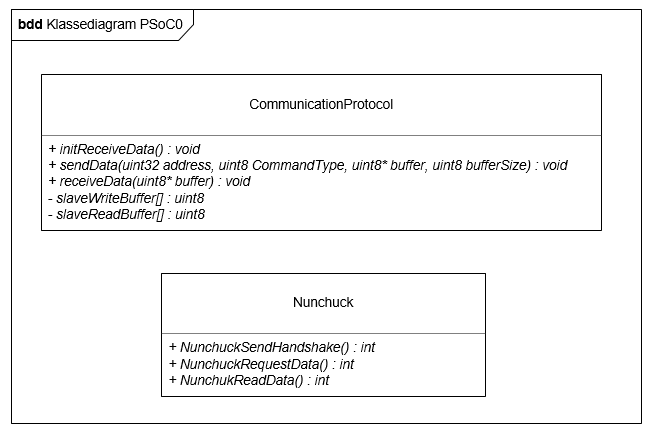
\includegraphics[width=\textwidth]{DesignOgImplementering/images/PSoC0KlasseDiagram}
	\caption{Klassediagram for CPU'en PSoC0}
	\label{figure:PSoC0KlasseDiagram}
\end{figure}

På figur \ref{figure:PSoC0KlasseDiagram} kan det ses at softwaren på PSoC0 CPU'en gør brug af klasserne \textit{CommunicationProtocol} samt \textit{Nunchuck}.

Klassebeskrivelser kan findes i \textbf{!INDSÆT BILAG TIL DOXYGEN!}

\subsection{Afkodning af Wii-Nunchuck Data Bytes}
Aflæste bytes fra Wii-Nunchuck - indeholdende tilstanden af knapperne og det analoge stick - er kodet når de oprindeligt modtages via I2C bussen. Disse bytes skal altså afkodes før deres værdier er brugbare. Afkodningen af hver byte sker ved brug af følgende formel:

\textit{AfkodetByte = (AflæstByte XOR 0x17) + 0x17}

Fra formlen kan det ses at den aflæste byte skal \textit{XOR}'s (Exclusive Or) med værdien 0x17, hvorefter dette resultat skal adderes med værdien 0x17.

\subsection{Kalibrering af Wii-Nunchuck Analog Stick}
De afkodede bytes for Wii-Nunchuck's analoge stick har definerede standardværdier for dets forskellige fysiske positioner. Disse værdier findes i tabel \ref{tabel:WiiNunchuckStickPositioner}

\begin{table}[H]
	\centering
	\begin{tabular}{|l|l|}
		\hline
		X-akse helt til venstre & 0x1E \\ \hline
		X-akse helt til højre   & 0xE1 \\ \hline
		X-akse centreret        & 0x7E \\ \hline
		Y-akse centreret        & 0x7B \\ \hline
		Y-akse helt frem        & 0x1D \\ \hline
		Y-akse helt tilbage     & 0xDF \\ \hline
	\end{tabular}
	\caption{Standardværdier for fysiske positioner af Wii-Nunchuck's analoge stick}
	\label{tabel:WiiNunchuckStickPositioner}
\end{table}

I praksis skal de afkodede værdier for det analoge stick kalibreres, da slør pga. brug gør at de ideale værdier ikke rammes. 

I projektet er de afkodede værdier for det analoge stick kalibreret med værdien -15 (0x0F i hexadecimal), altså ser den endelige formel for afkodning samt kalibrering således ud:

\textit{AfkodetByte = (AflæstByte XOR 0x17) + 0x17 - 0x0F}

\section{Hardwaredesign}
På baggrund af BDD'et er der fundet følgende hardwareblokke, der skal udarbejdes: 
\begin{itemize}
	\item Motorstyring
	\item Tre motorer
	\item Affyringsmekanisme 
\end{itemize}

\subsubsection{Motor}
Der er truffet et valg om at bruge en DC-motor i alle tre tilfælde. De to motorer skal bruges til at styre kanonen i to retninger, og den sidste skal bruges i affyringsmekanismen. 

\subsection{Motorstyring}
Til at styre de tre motorer er der bygget en H-bro, der skal bruges i tre eksemplarer. To af disse motorer skal kunne styre kanonen, så den ene gør at den kan køre op og ned, og den anden gør, at den kan køre fra side til side. Den tredje skal bruges til at styre affyringsmekanismen. 

\subsubsection{H-bro}
Der blev først designet en H-bro, som bestod af to N-MOSFET's af typen IRLZ44 og to P-MOSFET's af typen ZVP3306. Denne kan ses i bilaget. Det viste sig dog, at den P-MOSFET, der var brugt, var for svag til at kunne trække den strøm, som motoren skulle bruge, hvilket betød, at den blev brændt af. Derfor blev denne H-bro modificeret, så de to P-MOSFET's blev udskiftet med to MOSFET's af typen IRF9Z34N, der kan trække en større strøm. 

\begin{figure}[H]
	\centering
	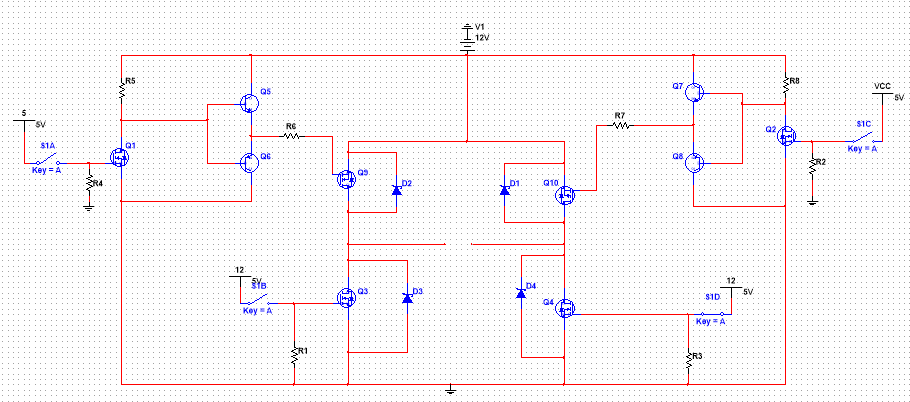
\includegraphics[width=\textwidth]{DesignOgImplementering/images/motorkreds}
	\caption{Kredsløb for H-bro}
	\end{figure}

\begin{table}[]
	\centering
	\caption{Komponentbetegnelser på H-bro}
	\label{my-label}
	\begin{tabular}{|l|l|l}
		\cline{1-2}
		Betegnelse 	& Komponent 	          	 &  \\ \cline{1-2}
		VCC        	& 5V                         &  \\ \cline{1-2}
		Q1   		& IRLZ44(mosfet N-Channel)   &  \\ \cline{1-2}
		Q2   		& IRLZ44(mosfet N-Channel)   &  \\ \cline{1-2}
		Q3   		& IRLZ44(mosfet N-Channel)   &  \\ \cline{1-2}
		Q4   		& IRLZ44(mosfet N-Channel)   &  \\ \cline{1-2}
		Q5   		& BC547                      &  \\ \cline{1-2}
		Q6   		& BC557                      &  \\ \cline{1-2}
		Q7   		& BC547                      &  \\ \cline{1-2}
		Q8   		& BC557                      &  \\ \cline{1-2}
		Q9   		& IRF9Z34N(mosfet P-Channel) &  \\ \cline{1-2}
		Q10  		& IRF9Z34N(mosfet P-Channel) &  \\ \cline{1-2}
		R1   		& 10k$\Omega$                &  \\ \cline{1-2}
		R2   		& 10k$\Omega$                &  \\ \cline{1-2}
		R3   		& 10k$\Omega$                &  \\ \cline{1-2}
		R4   		& 10k$\Omega$                &  \\ \cline{1-2}
		R5   		& 10k$\Omega$                &  \\ \cline{1-2}
		R6   		& 100$\Omega$                &  \\ \cline{1-2}
		R7   		& 100$\Omega$                &  \\ \cline{1-2}
		R8   		& 10k$\Omega$                &  \\ \cline{1-2}
		D1   		& IN5819                     &  \\ \cline{1-2}
		D2   		& IN5819                     &  \\ \cline{1-2}
		D3   		& IN5819                     &  \\ \cline{1-2}
		D4   		& IN5819                     &  \\ \cline{1-2}
	\end{tabular}
\end{table}

\subsubsection{MOSFET'er}
Til at styre motoren er der bygget en H-bro, som består af fire mosfet, hvor to af dem er af typen IRF9Z34N (mosfet P-channel, som er Q9 og Q10 på kredsløbstegningen) og de to andre mosfet er af typen IRLZ44 (mosfet N-Channel, som er Q3 og Q4 kredsløbstegningen). Det er valgt at bruge mosfet for at kunne styre H-broen, da det ved denne er muligt at lukke og åbne for spændingen, og de bliver styret af spænding, i forhold til transistorer, som bliver styret af strøm. 

\begin{itemize}
\item MOSFET N-kanal\\
	Der er i denne H-bro brugt en N-kanals-MOSFET af typen IRLZ44. Denne MOSFET skal bruges til at trække strømmen fra den tilsvarende P-MOSFET til stel, så motoren kan begynde at køre. Det sker, når der kommer 5V ind på gate-benet. 
	\\MOSFET'en fungerer på den måde, at når der kommer positiv spænding ind på gate-benet åbner den, så der kommer forbindelse til stel og når der kommmer 0V ind på dette lukker den igen. 
	
	\begin{figure}[H]
		\centering
		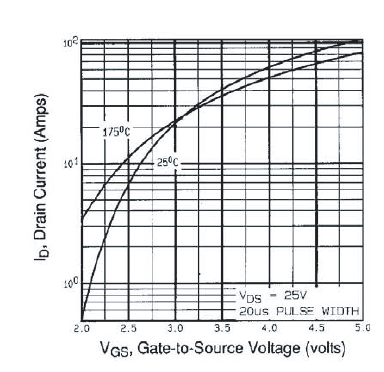
\includegraphics[width=\textwidth]{DesignOgImplementering/images/grafn}
		\caption{Gate-to-Source Voltage reference til datablad her!!!!}
	\end{figure}
	
	\\På figur (reference her!) ses det, at når der er en gate-to-source-spænding på 5V, vil der MOSFET'en kunne klare, at der løber en strøm på op til 100A/30A (TJEK DETTE!!). Det vil altså ikke komme til at påvirke motoren, da denne kun kan trække en strøm på cirka 0,35A. 
	
\item MOSFET P-kanal \\
	Der er valgt at bruge en P-MOSFET af typen IRF9Z34N. Denne MOSFET skal bruges til at trække de 12V ned til motoren, så denne kan køre. Samtidig sørger den for, at de 12V ikke løber ned til motoren så længe, der ikke er negativ spænding på gate-benet. 
	Denne kan trække en strøm på 6,7A ifølge databladet. Det vil altså ikke komme til at påvirke motoren, da den kun kan trække en strøm på cirka 0,35A. 
	
	For at der kan løbe spænding igennem IRF9Z34N (MOSFET P-channel), skal den have en negativ spænding for at åbne og en spænding på over 0V for at lukke. 
	hvor man kan se ved en Gate-to-Source voltage på 5v, vil der kunne 
	løbe en strøm på omkring 5A så det er mere end nok til at
	få motoren til at funger
	
	\begin{figure}[H]
		\centering
		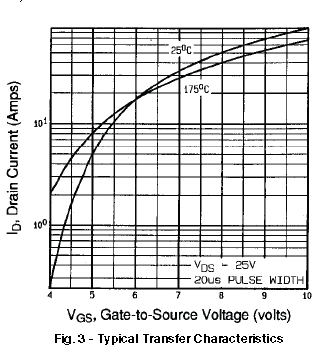
\includegraphics[width=\textwidth]{DesignOgImplementering/images/grafp}
		\caption{Gate-to-Source Voltag}
	\end{figure}
	så når mosfet får en negativ spædnding på ben(gate), vil den tillade at der kan løbe strøm/spænding
	igennem den og derved vil den ene del af kredsløbet blive aktiv, så motoren begynder at køre.
	så det er derfor at der er blevet sat to transistor og en N mosfet foran hver af P mosfetene.
\end{itemize}

\subsubsection{Dioder}
Over fire af mosfetene (Q9, Q10, Q3 og Q4) er der sat en diode af typen IN5819. Den skal fungere som beskyttelse af de fire mosfet (Q9, Q10, Q3 og Q4). Det, de gør, er, at de sikrer, at den spænding, som er tilbage i motoren, når man lukker for mosfetene, ikke løber tilbage ind i mosfetene og brænder dem af.

\subsubsection{Modstande}
\begin{itemize}
	\item Pull down modstande:\\
	Der er blevet brugt fire pull-down-modstande (R1, R2, R3 og R4). Disse sørger for, at signalet vil blive holdt lavt, når der ikke er trykket, så dette ben ikke står og flyver, så det kan komme til at åbne en mosfet ved en fejl og derved kommer til at brænde en mosfet eller motoren af. Der er valgt en modstand på 10 kOhm, hvilket betyder, at den er lille nok til at trække de små spændinger ned, når der ikke er trykket, og den stor nok til at spændingen ikke løber derned, når der er trykket. 
	\item Andre modstande
	\begin{itemize}
		\item R6 og R7\\
			Grunden til, at R6 og R7 er der, er for at sikre, at transistorernes Absolute Maximum Ratings omkring strømmen, som ikke må overstige 100mA ifølge databladet. (tjek lige om det er rigtig)
		\item R5 og R8\\
			Grunden til at R8 og R5 er der er, at der ikke kan løbe en alt for stor strøm igennem den N-mosfet, for ifølge databladet kan den kun klare en strøm på omkring 30A, når Vgs er på 10V, og da Vgs er sat til 5V, vil den ikke kunne klare en alt for stor strøm. Det vil altså sige, at er der R5 og R8 for at forhindre at N-mosfet brænder af.
	\end{itemize}

\end{itemize}

\subsubsection{Transistorer}
\begin{itemize}
	\item Q5 og Q7
	\item Q6 og Q8
\end{itemize}


